\documentclass[a4paper,11pt]{article}

% Identificação
\newcommand{\pbtitulo}{OpenKarel}
\newcommand{\pbversao}{1.0}

\usepackage{../sty/tutorial}

%----------------------------------------------------------------------
% Início do Documento
%----------------------------------------------------------------------
\begin{document}

\maketitle % mostrar o título
\thispagestyle{fancy} % habilitar o cabeçalho/rodapé das páginas

%-----------------------------------------------------------------------------
% RESUMO DO ARTIGO
%-----------------------------------------------------------------------------

\begin{abstract}
\initial{K}\textbf{arel é um robô que vive em um mundo com ruas, avenidas, paredes e sinalizadores. Seu principal objetivo é ensinar o pensamento computacional e programação de computadores. Karel possui um conjunto muito reduzido de comandos (apenas quatro), no qual é possível direcioná-lo para executar certas tarefas dentro do seu mundo e isso é uma parte muito importante no processo de aprendizado do estudante de programação que deve ensinar novos comandos a Karel de modo que possa extender suas capacidades e executar mais tarefas.}
\end{abstract}

%-----------------------------------------------------------------------------
% CONTEÚDO DO ARTIGO
%-----------------------------------------------------------------------------
\section{História de Karel e seu renascimento com OpenKarel}
Na década de 1970, um estudante de graduação de Stanford chamado \textbf{Rich Pattis} decidiu que seria mais fácil ensinar os fundamentos da programação se os alunos pudessem de alguma forma aprender as ideias básicas em um ambiente simples, livre das complexidades que caracterizam a maioria das linguagens de programação de alto nível. Inspirando-se do sucesso do projeto LOGO do Seymour Papert no MIT, Rich projetou um ambiente de programação introdutório no qual os alunos ensinam um robô a resolver problemas. Esse robô foi nomeado de Karel, o nome foi dado em homenagem ao escritor checo \textbf{Karel Capek}, que escreveu uma peça de teatro chamada R.U.R. (iniciais para "Rosumovi Univerzální Roboti"\cite{rur}) que deu origem a palavra robô na língua inglesa.
\begin{figure}[H]
	\centering
	
\includegraphics[width=0.2\textwidth]{imagem/logokarel.jpg}
	\caption{Logo de Karel}
\end{figure}

Karel foi um grande sucesso e usado em muitos cursos introdutórios de ciência da computação até o ponto em que o livro de Rich vendeu mais de 100.000 cópias. Muitas gerações de estudantes de CS106A\cite{cs106a} aprenderam como funciona a programação colocando Karel para resolver problemas criados pelos professores. Porém com o tempo a versão de Karel para Java ficou presa a versão 6.0 da Java SE.

Neste momento, por também adotar Karel nos cursos de Java para ensinar aos alunos, resolvi dar uma nova chance a este simpático robô e reconstruir seu ambiente no qual rebatizei de OpenKarel\cite{openkareloficial}. Foi adotado o comportamento idêntico ao original, porém com um número reduzido e simplificado de código fonte de modo que sua manutenção também pudesse ser simples e portátil para qualquer versão de Java.

\section{O Mundo de Karel}
O mundo de Karel é definido por \textbf{Ruas} (streets) que correm horizontalmente (leste-oeste) e \textbf{Avenidas} (avenues) que correm verticalmente (norte-sul). A cruzamento entre uma rua e de uma avenida é chamada \textbf{Esquina} (corner). Karel está sempre posicionado em uma determinada esquina e virado para uma das quatro direções padrão da bússola (norte, sul, leste, oeste). Um exemplo do mundo de Karel é mostrado abaixo. Na figura abaixo, Karel está localizado na esquina da 3ª rua e 4ª Avenida, voltado para leste.
\begin{figure}[H]
	\centering
	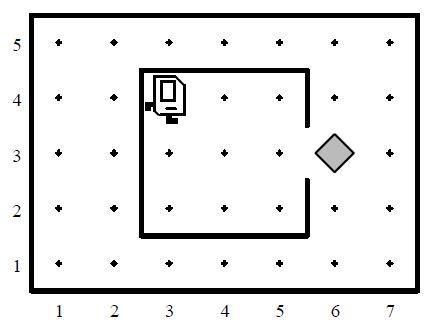
\includegraphics[width=0.6\textwidth]{imagem/mundo.jpg}
	\caption{Mundo de Karel}
\end{figure}

Vários outros componentes do mundo de Karel podem ser vistos neste exemplo. Cada ponto no mapa representa um esquina. O objeto na frente de Karel é um sinalizador (Beeper). Como descrito no livro de Rich Pattis, os sinalizadores são ``cones de plástico que emitem um barulho silencioso''. Karel só pode detectar um sinalizador se estiver em cima dele. As linhas contínuas no diagrama são paredes. As paredes servem como barreiras dentro do mundo de Karel. Karel não pode atravessar as paredes e o mundo de Karel também está sempre limitado por paredes ao longo das bordas, mas o mundo pode ter dimensões diferentes dependendo do problema específico que Karel precisa resolver.

Em muitos aspectos, Karel representa um ambiente ideal para ilustrar a abordagem orientada a objetos. Embora ninguém tenha realmente construído uma  implementação mecânica de Karel, é fácil imaginar Karel como um objeto do mundo real. Karel é, afinal, um robô, e os robôs são entidades do mundo real. As propriedades que definem o estado de Karel são sua localização no mundo, a direção que está enfrentando, e o número de sinalizadores em sua bolsa. 

\section{Programa de Karel}
Quando Karel foi introduzido na década de 1970, a abordagem predominante para escrever programas de computador foi o paradigma processual. Em grande parte, a programação processual é o processo de decomposição de um grande problema de programação em unidades menores, mais gerenciáveis, chamadas procedimentos que definem as operações necessárias. Embora a estratégia de quebrar programas em unidades menores permaneça uma parte vital de qualquer estilo de programação, as modernas linguagens como Java enfatizam uma abordagem diferente chamada paradigma Orientado a Objetos. Na programação Orientada a Objetos, a atenção do programador afasta-se da especificação procedural das operações e centra-se em modelar o comportamento de unidades conceitualmente integradas chamadas objetos. Objetos em uma linguagem de programação, por vezes, correspondem a objetos físicos no mundo real, mas como muitas vezes representam conceitos mais abstratos. A característica central de qualquer objeto - real ou abstrato - é o que faz sentido como um todo unificado.

A programação é muito uma atividade para se aprender na prática. O estudo da Ciência da Computação não é somente ler sobre algum conceito de programação. Coisas que parecem muito claras na página podem ser muito difíceis de se colocar em prática. Nessa sua nova implementação Orientada a Objetos, o estilo mais simples do programa Karel consiste na definição de uma nova classe Karel que especifica uma sequência de comandos internos que devem ser executados quando o programa é executado. Abaixo encontramos o esqueleto para o início de um programa OpenKarel:
\begin{lstlisting}
/**
 * Primeiro exemplo para OpenKarel
 * 
 * @author Fernando Anselmo
 * @version 1.0
 */

import openKarel.XKarel;

public class TstKarel extends XKarel {

    public static void main(String [] args) {
        new TstKarel();
    }
    
    public void run() {
        // Seus comandos aqui
    }
}
\end{lstlisting}

Este programa pode ser escrito em qualquer editor Java, porém recomendo fortemente o uso do BlueJ\cite{bluej} para o aluno iniciante. O BlueJ é um editor leve e por não possuir a complexidade dos editores profissionais torna-se o ambiente perfeito para o aprendizado. A disponibilização do OpenKarel neste editor é muito simples, primeiro obter a biblioteca ``openKarel.jar'' e no BlueJ acessar as opções "Tools | Preferences | Libraries" para disponibilizá-la para seus projetos.

As linhas entre /** e */ representam um comentário, que é simplesmente um texto concebido para explicar o funcionamento do programa para os leitores humanos. Em um programa simples, comentários extensos podem parecer bobagem pois o efeito do código pode ser óbvio, mas são extremamente importantes como um meio de descrever um projeto.

Agora começa o programa (em Java: a classe) em si, primeiro a importação da classe básica XKarel (todo programa Karel é uma extensão - termo da Orientação a Objetos que indica Herança - dessa classe). Quando uma classe é definida por extensão, a nova classe é dito ser uma subclasse do original. Neste exemplo, TstKarel é, portanto, uma subclasse (ou filha) de XKarel. O método inicial padrão de Java é o ``public static void main(String [] args)'' no qual é necessário para que este programa possa ser executado e ao fazê-lo criar um objeto da própria classe que responderá executando a seguinte janela:
\begin{figure}[H]
	\centering
	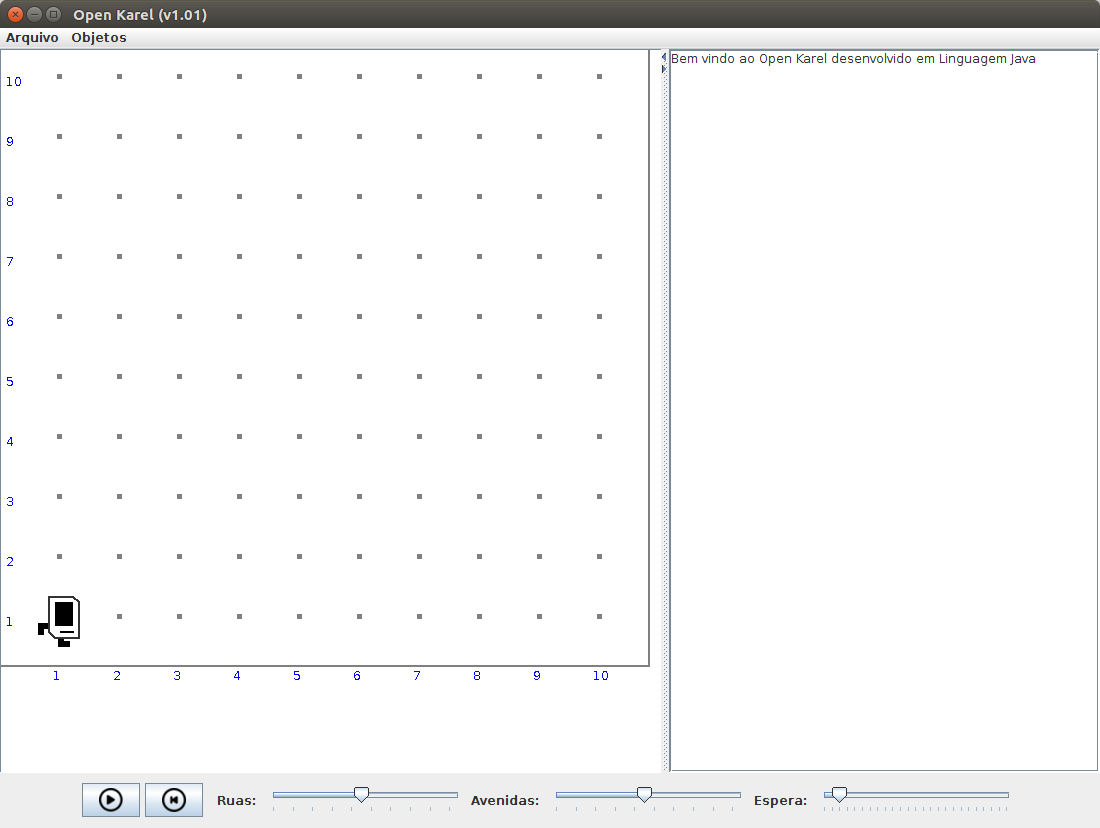
\includegraphics[width=0.6\textwidth]{imagem/janinicial.png}
	\caption{Janela Inicial}
\end{figure}

Ao ser iniciado o método run() será chamado e aonde está escrito: ``Seus comandos aqui'' é o local onde deve ser iniciado o programa para Karel. 
Originalmente, Karel pode responder aos seguintes comandos: \vspace{-1em}
\begin{itemize}
 \item move() - avançar uma esquina na direção em que estiver. Ocorrerá erro caso exista uma parede bloqueando seu caminho.
 \item turnLeft() - girar 90 graus para a esquerda (no sentido anti-horário).
 \item pickBeeper() - guardar o sinalizador que se encontra em sua posição na bolsa (que pode armazenar um número infinito de sinalizadores). Ocorrerá erro caso não exista um sinalizador na sua posição atual.
 \item putBeeper() - deixar um sinalizador de sua bolsa em sua posição atual. Ocorrerá erro caso não exista sinalizadores em sua bolsa.
\end{itemize} 

O comportamento de Karel é definido pelos comandos aos quais responde: move(), turnLeft(), pickBeeper() ou putBeeper(). O comando move() muda a localização e turnLeft() a direção de Karel, os dois restantes afetam tanto o número de sinalizadores em sua bolsa quanto ao número destes em seu mundo. \\[3mm]
O par vazio de parênteses que aparece em cada um desses métodos, parte da sintaxe comum compartilhada por Karel e Java, é usado para especificar uma chamada na qual não é necessário enviar nenhuma informação. Eventualmente, seus códigos podem incluir novas informações, mas essas informações não fazem parte do mundo inicial de Karel. \\[3mm]
Karel também pode responder aos seguintes questionamentos: \vspace{-1em}
\begin{itemize}
 \item frontIsClear() - Se a esquina a sua frente está vazia.
 \item leftIsClear() - Se a esquina a sua esquerda está vazia.
 \item rightIsClear() - Se a esquina a sua direita está vazia.
 \item beepersPresent() - Se existe um sinalizador em sua posição atual.
 \item beepersInBag() - Se existem sinalizadores em sua bolsa.
 \item facingNorth() - Se está virado para o Norte.
 \item facingEast() - Se está virado para o Leste.
 \item facingSouth() - Se está virado para o Sul.
 \item facingWest() - Se está virado para o Oeste.
 \item frontIsBlocked() - Se a esquina a sua frente está bloqueada.
 \item leftIsBlocked() - Se a esquina a sua esquerda está bloqueada
 \item rightIsBlocked() - Se a esquina a sua esquerda está bloqueada
 \item noBeepersPresent() - Se não existe um sinalizador em sua posição atual.
 \item noBeepersInBag() - Se não existem sinalizadores em sua bolsa.
 \item notFacingNorth() - Se não está virado para o Norte.
 \item notFacingEast() - Se não está virado para o Leste.
 \item notFacingSouth() - Se não está virado para o Sul.
 \item notFacingWest() - Se não está virado para o Oeste.
\end{itemize} 

A resposta de todos estes comandos é uma variável lógica indicando \textbf{true} (verdadeiro) ou \textbf{false} (falso) e através deles é possível avaliar as ações que devem ser tomadas para que Karel possa cumprir sua missão.

\subsection{Dicas finais antes dos desafios}
Ao programar Karel para executar uma determinada tarefa é necessário escrever os comandos de maneira precisa para que seja interpretado corretamente o que é necessário realizar. Os programas devem obedecer a um conjunto de regras e formato da Linguagem Original que Karel foi escrito, neste caso Java. Tomados em conjunto, os comandos predefinidos e as regras sintáticas definem a linguagem de programação Karel. Os programas de Karel possuem a mesma estrutura e envolvem os mesmos elementos fundamentais que os programas de Java. A diferença crítica é que a linguagem de programação de Karel é extremamente pequena, no sentido de ter muito poucos comandos e regras. É fácil, por exemplo, ensinar toda a linguagem Karel em apenas algumas horas, o que é realizado na CS106A. No final desse período, o aluno conhece tudo o que Karel pode fazer e como especificar essas ações em um programa. Os detalhes são fáceis de dominar e mesmo assim, é possivel resolver um problema que pode ser extremamente desafiador. A resolução de problemas é a essência da programação e as regras são apenas uma preocupação menor ao longo do caminho.

Como regra geral para as Instruções que devemos utilizar: \vspace{-1em}
\begin{enumerate}
  \item O programa deve ser capaz de trabalhar com comprimentos arbitrários. Não faz sentido conceber um programa que funciona apenas para mapas com um número predeterminado de ruas e avenidas. Em vez disso, crie programas que possam realizar a mesma tarefa em qualquer tipo de mapa. Tais programas, devem possuir a inteligência suficiente para reconhecer seu mundo.
  \item Uma passagem pode ocorrer em qualquer posição no mapa. Não deve haver limites para o número de passagens ou paredes bloqueando o caminho de Karel. Uma passagem é identificada por uma abertura na parede que representa a superfície do mapa.
  \item Passagens existentes já podem ter sido sinalizadas. Qualquer uma das passagens já pode conter um sinalizador deixado por uma equipe anterior de reparos. Nesse caso, Karel não deve colocar um sinal adicional.
  \item Criar novas funcionalidades para Karel. Crie métodos como turnRight(), putBeeperIsBeeperPresent(), entre outros, procure especializar as funcionalidades de Karel (por exemplo: Karel não sabe inicialmente virar a direita, que tal ensiná-lo?). 
  \item Regra Básica: Criar programas fáceis de ler, divida-os em curtos métodos ou em classes adicionais de modo a facilitar o máximo possível sua leitura.
\end{enumerate}

\section{Desafio 1 - Volta ao Mundo}
Karel é um robô que vive em seu mundo retangular com ``Avenidas'' (nas horizontais) e ``Ruas'' (nas verticais). OpenKarel é sua mais nova versão que 
permite rodar o programa em qualquer ambiente Java (antigamente estava limitado a versão Java SE 6.0) e assim é possível dar nova vida a Karel. \\[3mm]
Para iniciarmos na programação de Karel é necessário conhecermos alguns comandos de Java:

Comando de Decisão SE, em Java é reconhecido pela palavra chave \textbf{if} e sua estrutura é a seguinte:
\begin{lstlisting}
if (decisao_logica) {
  instrucoes_caso_verdadeiro;
}
\end{lstlisting}

Comando de Repetição PARA, em Java é reconhecido pela palavra chave \textbf{for} e sua estrutura é a seguinte:
\begin{lstlisting}
for (variavel_inicial; decisao_logica; incremento) {
  instrucoes_caso_verdadeiro;
}
\end{lstlisting}

Comando de Repetição ENQUANTO, em Java é reconhecido pela palavra chave \textbf{while} e sua estrutura é a seguinte:
\begin{lstlisting}
while (decisao_logica) {
  instrucoes_caso_verdadeiro;
}
\end{lstlisting}

Outro detalhe que devemos nos ater na lógica de Karel é a necessidade de construirmos métodos para realizarmos as ações e não mantermos tudo fechado dentro do método principal de execução (run). Um método em Java possui a seguinte estrutura:
\begin{lstlisting}
[modificador] retorno nome_metodo([parametros]) {
  instrucoes_do_metodo;
}
\end{lstlisting}

O tipo da variável de retorno de um método é sempre obrigatório, caso não retorne nada, a palavra chave \textbf{void} é usada nesta posição.

Agora podemos começar a escrever nosso primeiro programa, crie uma nova classe para este desafio (por exemplo: RodaMundo) e siga o esqueleto descrito para o início dessa. Para que Karel dê a volta completa em seu mundo, devemos escrever dentro do método \textbf{run()} desta classe as seguintes instruções:
\begin{lstlisting}
public void run() {
  for (byte i = 0; i < 4; i++) {
    for (byte j = 0; j < 9; j++) {
      move();
    }
    turnLeft();
  }
}
\end{lstlisting}

Sendo que o primeiro laço ``for'' seria usado para repetir 4 vezes a execução de mover 9 vezes e virar a esquerda. Execute esta classe e observe que isso só serviria se o mundo tivesse obrigatoriamente 10 Avenidas por 10 Ruas. Então o ideal seria primeiro criar um método que Karel ao tentar andar nos responda se conseguiu ou não, conforme a seguinte codificação:
\begin{lstlisting}
public boolean andar() {
  if (frontIsClear()) {
    move();
    return true;
  }
  return false;
}
\end{lstlisting}

Neste método Karel verifica se não há qualquer obstáculo a sua frente, caso não haja realiza o movimento e nos devolve ``verdadeiro'' (true) como resposta, caso haja obstáculo retorna ``falso'' (false). Modificaremos o método \textbf{run()} para:
\begin{lstlisting}
public void run() {
  for (byte i = 0; i < 4; i++) {
    while (andar());
    turnLeft();
  }
}
\end{lstlisting}

Pronto, agora Karel consegue percorrer ao redor de seu mundo sem qualquer problema, execute o código aumentando ou diminuindo o número de Avenidas e Ruas e 
perceba que tudo está OK.

Agora é sua vez, imagine que no caminho de Karel existam sinalizadores, não sabemos em qual esquina eles se encontram nem quantos são, mas sabemos que estão 
no caminho que Karel percorre, modifique o programa de modo que Karel possa recolher todos os que encontrar.

\section{Conclusão}
Karel é uma ferramenta que promove um convívio harmônico entre a criatividade e a lógica de uma maneira coerente. Pode ser extremamente útil para construir uma forte base de aprendizado a programação de computadores. Partindo que suas instruções iniciais são muitos simples de serem absorvidas por qualquer um e com pouquíssimos passos é possível realizar várias ações, só que para isso requer do aluno um profundo estudo e dedicação.

Programar em uma linguagem como JAVA, requer meses de treinamento e prática, porém Karel pode ajudar a encurtar esse período e auxiliar a como dar um passo atrás de outro, o melhor caminho a seguir, como realizar comandos de decisão e laços de repetição, e qual o melhor processo para a resolução de um determinado problema. Karel é um Robô simples que vive em um mundo simples. Devido que Karel e seu mundo são simuladores, podemos realmente ver os resultados de uma programação em ação. 

Sou um entusiasta do mundo \textbf{Open Source} e novas tecnologias. Qual a diferença entre Livre e Open Source? \underline{Livre} significa que esta apostila é gratuita e pode ser compartilhada a vontade. \underline{Open Source} além de livre todos os arquivos que permitem a geração desta (chamados de arquivos fontes) devem ser disponibilizados para que qualquer pessoa possa modificar ao seu prazer, gerar novas, complementar ou fazer o que quiser. Os fontes da apostila (que foi produzida com o LaTex) está disponibilizado no GitHub\cite{github}, assim baixar, alterar e usar. Veja ainda outros artigos que publico sobre tecnologia através do meu Blog Oficial\cite{fernandoanselmo}.

%-----------------------------------------------------------------------------
% REFERÊNCIAS
%-----------------------------------------------------------------------------
\begin{thebibliography}{7}
  \bibitem{rur} 
  A peça conta a história de um brilhante cientista, chamado Rossum, que desenvolve uma substância química similar ao protoplasma. Utiliza essa substância para construção de humanoides (robôs), com o intuito de que estes sejam obedientes e realizem todo o trabalho físico.

  \bibitem{cs106a} 
  Curso de Metodologia da programação de Stanford \\
  \url{https://see.stanford.edu/Course/CS106A}
  
  \bibitem{openkareloficial} 
  Página do OpenKarel no GitHub \\
  \url{https://github.com/fernandoans/OpenKarel}
  
  \bibitem{bluej} 
  Editor BlueJ para Java \\
  \url{http://bluej.org/}

  \bibitem{fernandoanselmo} 
  Fernando Anselmo - Blog Oficial de Tecnologia \\
  \url{http://www.fernandoanselmo.blogspot.com.br/}
  
  \bibitem{publicacao} 
  Encontre essa e outras publicações em \\
  \url{https://cetrex.academia.edu/FernandoAnselmo}

  \bibitem{github} 
  Repositório para os fontes da apostila \\
  \url{https://github.com/fernandoans/publicacoes}
\end{thebibliography}
  
\end{document}
